\hypertarget{what-is-the-concurrent-system-architecture-that-will-be-used-in-this-paper}{%
\section{What is the concurrent system architecture that will be used in
this
paper}\label{what-is-the-concurrent-system-architecture-that-will-be-used-in-this-paper}}

This paper assumes the reader is familiar with Concurrency, LTS, LTSA
and FSP.

In this paper two implementations of a finite-state machine will be
used:

\begin{itemize}
\tightlist
\item
  Device-driver, communicate with external devices
\item
  Thread, making decisions about the system
\end{itemize}

They both follow from a FSP design, however they differ in their way of
making transitions.

When a Thread makes a transition the following steps are taken:

\begin{itemize}
\tightlist
\item
  Execute an action
\item
  Changing the current state according to the FSP design
\item
  Setting its sensitivity-list according to the FSP design and the
  current state
\end{itemize}

When a device-driver makes a transition the slightly differ, this is
because the device-driver communicates with external devices and based
upon these external devices in combination with its current state and
FSP design will it determine its sensitivity-list. The steps are:

\begin{itemize}
\tightlist
\item
  Execute an action
\item
  Change the current state according to the FSP design
\item
  Setting its sensitivity-list according to the external devices, FSP
  design and the current state
\end{itemize}

Determining the action that will be executed by the finite-state
machines is done by the synchronization-server. Based upon the
sensitivity-lists and alphabets of the processes it will determine the
next action that will be executed and which of the processes will
execute this action.

The described elements are shown in the following diagram, this diagram
represents the concurrent system architecture.

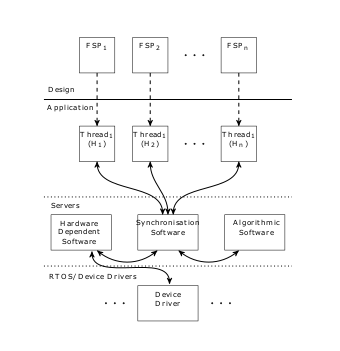
\includegraphics{../img/system_architecture.png} //Add reference

In the top of the diagram are the threads shown, they are represented by
FSP models. At the bottom of the diagram the device-drivers are shown.

At the center of the diagram is the synchronization-server shown, it
allows communication between device-drivers and threads.

The algorithmic software located on the center right is not used in this
paper.
